\chapter{Simulation und Auswertung}\label{chap:simulation}

\noindent
Dieses Kapitel beschreibt die Durchführung von Simulationen und die Auswertung der Ergebnisse. Es umfasst die Definition von Messgrößen, Akzeptanzkriterien und die Aufbereitung der Ergebnisse für die Analyse. Die Simulation von E/E-Architekturen erfordert eine sorgfältige Modellierung der verschiedenen Systemkomponenten und deren Interaktionen \cite{network_simulation, simulation_automotive}. Moderne Simulationsansätze für Fahrzeugsysteme werden in \cite{simulation_automotive, validation_verification} ausführlich beschrieben.

\section{Messgrößen}

Die Messgrößen werden für moderne E/E-Architekturen mit neuesten Sensoren (Bosch 8MP Multifunktionskamera) und Rechenplattformen (NVIDIA DRIVE Thor) definiert. Diese Komponenten stellen neue Anforderungen an die Metriken und deren Messung.

\subsection{Timing-Metriken}

\subsubsection{End-to-End-Latenz}

Die End-to-End-Latenz (E2E-Latenz) misst die Zeit von der Erzeugung eines Signals an einem Sensor bis zur Ankunft am Aktor. Diese Metrik ist von zentraler Bedeutung für sicherheitskritische Funktionen, da sie direkt die Reaktionszeit des Systems bestimmt \cite{real_time_systems, automated_driving_systems}.

Die E2E-Latenz setzt sich aus mehreren Komponenten zusammen:

\begin{equation}
L_{E2E} = L_{sensor} + L_{network1} + L_{processing1} + L_{network2} + L_{processing2} + \ldots + L_{networkN} + L_{actuator}
\end{equation}

wobei:
\begin{itemize}
  \item $L_{sensor}$: Sensor-Verarbeitungszeit (Bildaufnahme, Signalaufbereitung)
  \item $L_{networki}$: Netzwerk-Latenz für Link $i$ (Serialisierung, Propagation, Queueing, Switching)
  \item $L_{processingi}$: Verarbeitungszeit auf ECU $i$ (Task-Ausführung, Scheduling-Verzögerung)
  \item $L_{actuator}$: Aktor-Reaktionszeit
\end{itemize}

\begin{itemize}
  \item \textbf{Messung}: Zeitstempel am Sensor vs. Zeitstempel am Aktor
    \begin{itemize}
      \item Synchronisierte Zeitstempel durch TSN gPTP-Synchronisation
      \item Präzision: Mikrosekunden-Genauigkeit für TSN-Netze
      \item Messung für jedes Frame/Signal in der Chain
    \end{itemize}
  
  \item \textbf{Statistiken}: Min, Max, Mean, Median, 95. Perzentil, 99. Perzentil
    \begin{itemize}
      \item \textbf{Min}: Best-Case-Latenz (wichtig für Optimierung)
      \item \textbf{Max}: Worst-Case-Latenz (kritisch für Deadline-Prüfung)
      \item \textbf{Mean}: Durchschnittliche Latenz (für Performance-Bewertung)
      \item \textbf{Median}: Typische Latenz (weniger empfindlich gegen Outlier)
      \item \textbf{95./99. Perzentil}: Latenz, die in 95\%/99\% der Fälle nicht überschritten wird
    \end{itemize}
  
  \item \textbf{Chain-spezifisch}: Latenz für jede Funktionskette separat
    \begin{itemize}
      \item Jede Chain hat eigene E2E-Latenz-Anforderungen
      \item Kritische Chains (z.\,B. Lenkung, Bremse) haben strikte Deadlines (< 100 ms)
      \item Nicht-kritische Chains (z.\,B. Infotainment) haben weniger strikte Anforderungen
    \end{itemize}
  
  \item \textbf{Ziel}: Prüfung, ob Deadlines eingehalten werden
    \begin{itemize}
      \item Vergleich der gemessenen E2E-Latenz mit der definierten Deadline
      \item Identifikation von Chains, die ihre Deadlines nicht einhalten
      \item Analyse der Latenz-Komponenten zur Identifikation von Bottlenecks
    \end{itemize}
\end{itemize}

\begin{figure}[h]
  \centering
  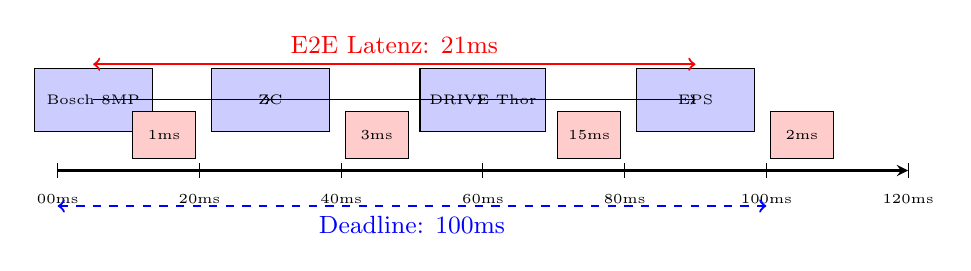
\begin{tikzpicture}[
    scale=0.9,
    timeline/.style={thick, -stealth},
    component/.style={rectangle, draw, fill=blue!20, minimum width=1.5cm, minimum height=0.8cm, text centered, font=\tiny},
    latency/.style={rectangle, draw, fill=red!20, minimum width=0.8cm, minimum height=0.6cm, text centered, font=\tiny}
  ]
    % Timeline
    \draw[timeline] (0,0) -- (12,0);
    \foreach \x in {0,2,4,6,8,10,12} {
      \draw (\x, -0.1) -- (\x, 0.1);
      \node[below, font=\tiny] at (\x, -0.2) {\x0ms};
    }
    
    % Components
    \node[component] at (0.5, 1) {Bosch 8MP};
    \node[component] at (3, 1) {ZC};
    \node[component] at (6, 1) {DRIVE Thor};
    \node[component] at (9, 1) {EPS};
    
    % Latencies
    \node[latency] at (1.5, 0.5) {1ms};
    \node[latency] at (4.5, 0.5) {3ms};
    \node[latency] at (7.5, 0.5) {15ms};
    \node[latency] at (10.5, 0.5) {2ms};
    
    % Arrows
    \draw[->] (0.5, 1) -- (3, 1);
    \draw[->] (3, 1) -- (6, 1);
    \draw[->] (6, 1) -- (9, 1);
    
    % E2E annotation
    \draw[<->, thick, red] (0.5, 1.5) -- (9, 1.5) node[midway, above, font=\small] {E2E Latenz: 21ms};
    \draw[<->, thick, blue, dashed] (0, -0.5) -- (10, -0.5) node[midway, below, font=\small] {Deadline: 100ms};
  \end{tikzpicture}
  \caption{Beispiel: E2E-Latenz-Zerlegung für eine Funktionskette}
  \label{fig:e2e_latency}
\end{figure}

\subsubsection{Jitter}

Jitter misst die Variabilität der Latenz:

\begin{itemize}
  \item \textbf{Definition}: Standardabweichung oder Differenz zwischen Max und Min
  \item \textbf{Chain-spezifisch}: Jitter für jede Chain
  \item \textbf{Ziel}: Prüfung der Deterministik
\end{itemize}

\subsubsection{Deadline-Misses}

Deadline-Misses zählen, wie oft Deadlines verletzt werden:

\begin{itemize}
  \item \textbf{Task-Deadlines}: Anzahl verpasster Task-Deadlines
  \item \textbf{Frame-Deadlines}: Anzahl verpasster Frame-Deadlines
  \item \textbf{Chain-Deadlines}: Anzahl verpasster E2E-Deadlines
  \item \textbf{Ziel}: Identifikation von Timing-Problemen
\end{itemize}

\subsection{Kommunikations-Metriken}

\subsubsection{Busauslastung}

Die Busauslastung misst die Bandbreiten-Nutzung:

\begin{itemize}
  \item \textbf{Link-spezifisch}: Auslastung für jeden Link
  \item \textbf{Switch-spezifisch}: Auslastung für jeden Switch-Port
  \item \textbf{Statistiken}: Min, Max, Mean über Zeit
  \item \textbf{Ziel}: Identifikation von Bandbreiten-Bottlenecks
\end{itemize}

\subsubsection{Paketverluste}

Paketverluste zählen verlorene oder verworrene Pakete:

\begin{itemize}
  \item \textbf{Ursachen}: Queue-Überlauf, Fehler, Timeouts
  \item \textbf{Frame-spezifisch}: Verluste für jeden Frame-Typ
  \item \textbf{Link-spezifisch}: Verluste für jeden Link
  \item \textbf{Ziel}: Prüfung der Zuverlässigkeit
\end{itemize}

\subsubsection{Queue-Längen}

Queue-Längen messen die Warteschlangen-Größe:

\begin{itemize}
  \item \textbf{Switch-Queues}: Länge für jede Queue an jedem Switch
  \item \textbf{Statistiken}: Max, Mean, 95. Perzentil
  \item \textbf{Ziel}: Identifikation von Überlastungen
\end{itemize}

\subsection{Ressourcen-Metriken}

\subsubsection{CPU/GPU-Last}

Die CPU/GPU-Last misst die Prozessor-Auslastung:

\begin{itemize}
  \item \textbf{ECU-spezifisch}: Last für jeden ECU
  \item \textbf{Task-spezifisch}: Last für jeden Task
  \item \textbf{Statistiken}: Min, Max, Mean über Zeit
  \item \textbf{Ziel}: Identifikation von CPU-Bottlenecks
\end{itemize}

\subsubsection{Wartezeiten}

Wartezeiten messen, wie lange Tasks auf CPU-Zeit warten:

\begin{itemize}
  \item \textbf{Task-spezifisch}: Wartezeit für jeden Task
  \item \textbf{Statistiken}: Max, Mean, 95. Perzentil
  \item \textbf{Ziel}: Identifikation von Scheduling-Problemen
\end{itemize}

\subsubsection{Speicher-Auslastung}

Die Speicher-Auslastung misst die RAM-Nutzung:

\begin{itemize}
  \item \textbf{ECU-spezifisch}: Speicher für jeden ECU
  \item \textbf{Task-spezifisch}: Speicher für jeden Task
  \item \textbf{Ziel}: Prüfung von Speicher-Überläufen
\end{itemize}

\subsection{Verfügbarkeits-Metriken}

\subsubsection{MTBF}

Mean Time Between Failures (MTBF) misst die durchschnittliche Zeit zwischen Ausfällen:

\begin{itemize}
  \item \textbf{Komponenten-spezifisch}: MTBF für jede Komponente
  \item \textbf{System-MTBF}: Gesamt-MTBF des Systems
  \item \textbf{Ziel}: Bewertung der Zuverlässigkeit
\end{itemize}

\subsubsection{Verfügbarkeit}

Die Verfügbarkeit misst den Anteil der Zeit, in der das System funktionsfähig ist:

\begin{equation}
A = \frac{MTBF}{MTBF + MTTR}
\end{equation}

wobei MTTR die Mean Time To Repair ist.

\subsubsection{Downtime}

Downtime misst die Zeit, in der das System nicht funktionsfähig ist:

\begin{itemize}
  \item \textbf{Total Downtime}: Gesamte Ausfallzeit
  \item \textbf{Number of Failures}: Anzahl der Ausfälle
  \item \textbf{Ziel}: Bewertung der Fehlertoleranz
\end{itemize}

\subsection{Energie-Metriken}

\subsubsection{Energieverbrauch}

Der Energieverbrauch misst den Stromverbrauch:

\begin{itemize}
  \item \textbf{ECU-spezifisch}: Energie für jeden ECU
  \item \textbf{Power-State-spezifisch}: Energie in jedem Power State
  \item \textbf{System-Energie}: Gesamt-Energieverbrauch
  \item \textbf{Ziel}: Bewertung der Energieeffizienz
\end{itemize}

\subsubsection{Power-State-Verteilung}

Die Power-State-Verteilung zeigt, wie viel Zeit in jedem Zustand verbracht wird:

\begin{itemize}
  \item \textbf{Duty-Cycle}: Anteil der Zeit in jedem State
  \item \textbf{Übergänge}: Anzahl der State-Übergänge
  \item \textbf{Ziel}: Optimierung der Energieeffizienz
\end{itemize}

\section{Akzeptanzkriterien}

\subsection{OEM/Normen-basierte Grenzwerte}

\subsubsection{Timing-Anforderungen}

\begin{table}[h]
  \centering
  \caption{Beispiel: Timing-Anforderungen für verschiedene Funktionen}
  \begin{tabular}{lll}
    \toprule
    Funktion & E2E-Latenz & Jitter \\
    \midrule
    Notbremsung (AEB) & < 100 ms & < 10 ms \\
    Lenkung (LKA) & < 150 ms & < 20 ms \\
    ACC & < 200 ms & < 30 ms \\
    Infotainment & < 500 ms & < 50 ms \\
    \bottomrule
  \end{tabular}
  \label{tab:timing_anforderungen}
\end{table}

\subsubsection{Sicherheitsanforderungen}

\begin{itemize}
  \item \textbf{ASIL D}: Verfügbarkeit > 99.9\%
  \item \textbf{ASIL C}: Verfügbarkeit > 99.5\%
  \item \textbf{ASIL B}: Verfügbarkeit > 99\%
  \item \textbf{ASIL A}: Verfügbarkeit > 95\%
\end{itemize}

\subsection{TSN-Latenz-/Jitter-Budgets}

Für TSN-Netze gelten spezielle Budgets:

\begin{itemize}
  \item \textbf{Kritische Frames}: Latenz < 1 ms, Jitter < 0.1 ms
  \item \textbf{Standard-Frames}: Latenz < 10 ms, Jitter < 1 ms
  \item \textbf{Best-Effort}: Keine Garantien
\end{itemize}

\subsection{Performance-Ziele}

\begin{itemize}
  \item \textbf{CPU-Auslastung}: < 80\% für Safety-kritische ECUs
  \item \textbf{Netzwerk-Auslastung}: < 70\% für kritische Links
  \item \textbf{Paketverluste}: < 0.1\% für kritische Frames
  \item \textbf{Deadline-Misses}: 0 für Safety-kritische Tasks
\end{itemize}

\section{Ergebnisaufbereitung}

\subsection{Dashboards}

\subsubsection{Python/Plotly-Dashboards}

Interaktive Dashboards werden mit Python und Plotly erstellt:

\begin{itemize}
  \item \textbf{Timing-Dashboard}: E2E-Latenzen, Jitter, Deadline-Misses
  \item \textbf{Kommunikations-Dashboard}: Busauslastung, Paketverluste, Queue-Längen
  \item \textbf{Ressourcen-Dashboard}: CPU/GPU-Last, Speicher-Auslastung
  \item \textbf{Verfügbarkeits-Dashboard}: MTBF, Verfügbarkeit, Downtime
  \item \textbf{Energie-Dashboard}: Energieverbrauch, Power-State-Verteilung
\end{itemize}

\subsubsection{Visualisierungen}

\begin{itemize}
  \item \textbf{Zeitreihen}: Entwicklung von Metriken über Zeit
  \item \textbf{Histogramme}: Verteilung von Latenzen, Jitter
  \item \textbf{Heatmaps}: Auslastung über verschiedene Komponenten
  \item \textbf{Network-Graphs}: Topologie mit annotierten Metriken
\end{itemize}

\subsection{Variantenvergleich}

\subsubsection{Multi-Variant-Analyse}

Verschiedene Design-Varianten werden verglichen:

\begin{itemize}
  \item \textbf{Tabellarischer Vergleich}: Metriken für jede Variante
  \item \textbf{Spider-Diagramme}: Multi-Kriterien-Vergleich
  \item \textbf{Pareto-Front}: Trade-offs zwischen verschiedenen Zielen
\end{itemize}

\subsubsection{Statistische Analyse}

\begin{itemize}
  \item \textbf{Signifikanz-Tests}: Prüfung, ob Unterschiede signifikant sind
  \item \textbf{Confidence-Intervals}: Konfidenzintervalle für Metriken
  \item \textbf{Sensitivitäts-Analyse}: Identifikation kritischer Parameter
\end{itemize}

\subsection{Trace-basierte Analysen}

\subsubsection{Event-Traces}

Event-Traces zeigen die zeitliche Abfolge von Ereignissen:

\begin{itemize}
  \item \textbf{Task-Ausführungen}: Wann Tasks starten/enden
  \item \textbf{Frame-Übertragungen}: Wann Frames gesendet/empfangen werden
  \item \textbf{State-Übergänge}: Power-State-Übergänge, Fehler-Ereignisse
\end{itemize}

\subsubsection{Critical-Path-Analyse}

Der Critical Path identifiziert den längsten Pfad durch das System:

\begin{itemize}
  \item \textbf{Chain-Analyse}: Welche Chain hat die längste Latenz?
  \item \textbf{Bottleneck-Identifikation}: Welche Komponente verursacht die Verzögerung?
  \item \textbf{Optimierungs-Vorschläge}: Wo kann optimiert werden?
\end{itemize}

\subsubsection{Timing-Diagramme}

Timing-Diagramme visualisieren die zeitliche Abfolge:

\begin{itemize}
  \item \textbf{Gantt-Charts}: Task-Ausführungen über Zeit
  \item \textbf{Sequence-Diagrams}: Kommunikation zwischen Komponenten
  \item \textbf{State-Diagrams}: State-Übergänge über Zeit
\end{itemize}

\section{Erweiterte Simulations-Beispiele}

Dieser Abschnitt präsentiert erweiterte Beispiele für die Simulation und Auswertung von E/E-Architekturen. Die Beispiele zeigen, wie verschiedene Szenarien simuliert und ausgewertet werden können.

\subsection{Beispiel: Komplexe Multi-Sensor-Perzeption}

Dieses Beispiel zeigt die Simulation einer komplexen Perzeptions-Pipeline mit mehreren Sensoren:

\subsubsection{Architektur}

\begin{itemize}
  \item \textbf{Sensoren}:
    \begin{itemize}
      \item 3x Front-Kameras (Stereo + Mono)
      \item 2x Radar (Kurz- und Langstrecke)
      \item 1x LiDAR (64-Layer)
      \item 8x Ultraschall-Sensoren
    \end{itemize}
  
  \item \textbf{Verarbeitung}:
    \begin{itemize}
      \item Bildverarbeitung auf ZC\_Front (3x Kamera-Streams)
      \item Radar-Signalverarbeitung auf ZC\_Front
      \item LiDAR-Verarbeitung auf ZC\_Front
      \item Sensorfusion auf AD-DC
      \item Objekterkennung und Tracking auf AD-DC
    \end{itemize}
  
  \item \textbf{Kommunikation}:
    \begin{itemize}
      \item Kamera-Streams: Ethernet 1 Gbps, 30 fps, 1500 Byte/Frame
      \item Radar-Daten: CAN-FD, 20 Hz, 64 Byte/Frame
      \item LiDAR-Daten: Ethernet 2.5 Gbps, 10 Hz, 100 KB/Frame
      \item Fused Data: TSN Priority 6, 30 Hz
    \end{itemize}
\end{itemize}

\subsubsection{Simulations-Ergebnisse}

Typische Ergebnisse für dieses Szenario:

\begin{table}[h]
  \centering
  \caption{Simulations-Ergebnisse: Multi-Sensor-Perzeption}
  \begin{tabular}{lll}
    \toprule
    Metrik & Wert & Kommentar \\
    \midrule
    E2E-Latenz (Mean) & 45 ms & Innerhalb Budget \\
    E2E-Latenz (Max) & 78 ms & Innerhalb Deadline (100 ms) \\
    Jitter & 8 ms & Akzeptabel \\
    CPU-Last (ZC\_Front) & 65\% & Moderate Last \\
    CPU-Last (AD-DC) & 72\% & Hohe Last, aber OK \\
    GPU-Last (AD-DC) & 58\% & Moderate Last \\
    Netzwerk-Last (Ethernet) & 52\% & Moderate Last \\
    Paketverluste & 0.01\% & Sehr niedrig \\
    \bottomrule
  \end{tabular}
  \label{tab:multisensor_results}
\end{table}

\subsection{Beispiel: Stress-Test unter extremer Last}

Dieses Beispiel zeigt die Simulation unter extremer Last (Stau-Szenario):

\subsubsection{Szenario-Parameter}

\begin{itemize}
  \item \textbf{Objektdichte}: 80 Objekte in Szene
  \item \textbf{Simulationsdauer}: 20 Minuten
  \item \textbf{Geschwindigkeit}: 0-20 km/h (Stau)
  \item \textbf{Ziel}: Prüfung, ob Deadlines auch unter extremer Last eingehalten werden
\end{itemize}

\subsubsection{Ergebnisse}

\begin{table}[h]
  \centering
  \caption{Stress-Test Ergebnisse}
  \begin{tabular}{lll}
    \toprule
    Metrik & Wert & Status \\
    \midrule
    E2E-Latenz (Max) & 112 ms & \textcolor{red}{Über Deadline (100 ms)} \\
    Deadline-Misses & 2.3\% & \textcolor{red}{Nicht akzeptabel} \\
    CPU-Last (Peak) & 92\% & \textcolor{red}{Sehr hoch} \\
    Netzwerk-Last (Peak) & 78\% & \textcolor{orange}{Hoch} \\
    Queue-Überläufe & 15 & \textcolor{red}{Problematisch} \\
    \bottomrule
  \end{tabular}
  \label{tab:stress_test_results}
\end{table}

\subsubsection{Analyse und Optimierung}

Die Ergebnisse zeigen, dass Optimierungen erforderlich sind:

\begin{itemize}
  \item \textbf{CPU-Bottleneck}: Die CPU-Auslastung ist zu hoch
    \begin{itemize}
      \item Lösung: Optimierung der Objekterkennungs-Algorithmen
      \item Alternative: Zusätzliche CPU-Kerne oder höhere Taktfrequenz
    \end{itemize}
  
  \item \textbf{Netzwerk-Bottleneck}: Die Netzwerk-Auslastung ist hoch
    \begin{itemize}
      \item Lösung: Erhöhung der Bandbreite (1 Gbps $\rightarrow$ 2.5 Gbps)
      \item Alternative: Kompression der Sensor-Daten
    \end{itemize}
  
  \item \textbf{Deadline-Misses}: Einige Deadlines werden verpasst
    \begin{itemize}
      \item Lösung: Priorisierung kritischer Tasks
      \item Alternative: Reduzierung der Objektdichte durch Filterung
    \end{itemize}
\end{itemize}

\section{Erweiterte Auswertungs-Methoden}

Dieser Abschnitt beschreibt erweiterte Methoden zur Auswertung von Simulationsergebnissen.

\subsection{Statistische Analyse}

Statistische Methoden ermöglichen eine fundierte Analyse der Ergebnisse:

\subsubsection{Verteilungsanalyse}

Die Verteilung von Metriken wird analysiert:

\begin{itemize}
  \item \textbf{Normalverteilung}: Prüfung auf Normalverteilung (Shapiro-Wilk-Test)
  \item \textbf{Andere Verteilungen}: Weibull, Exponential, etc.
  \item \textbf{Outlier-Erkennung}: Identifikation von Ausreißern (IQR-Methode, Z-Score)
  \item \textbf{Perzentile}: Berechnung von Perzentilen (P50, P95, P99)
\end{itemize}

\subsubsection{Korrelationsanalyse}

Korrelationen zwischen Metriken werden analysiert:

\begin{itemize}
  \item \textbf{Pearson-Korrelation}: Lineare Korrelationen
  \item \textbf{Spearman-Korrelation}: Monotone Korrelationen
  \item \textbf{Korrelations-Matrix}: Visualisierung von Korrelationen
  \item \textbf{Kausalitäts-Analyse}: Identifikation von Kausalzusammenhängen
\end{itemize}

\subsection{Machine-Learning-basierte Analyse}

ML-Methoden können für erweiterte Analysen verwendet werden:

\begin{itemize}
  \item \textbf{Clustering}: Identifikation von ähnlichen Szenarien
  \item \textbf{Anomalie-Erkennung}: Automatische Erkennung von Anomalien
  \item \textbf{Prädiktion}: Vorhersage von Metriken basierend auf Parametern
  \item \textbf{Feature-Importance}: Identifikation wichtiger Parameter
\end{itemize}

\section{Erweiterte Simulations-Beispiele}

Dieser Abschnitt präsentiert detaillierte Beispiele für Simulationsergebnisse.

\subsection{Beispiel: Detaillierte E2E-Latenz-Analyse}

\subsubsection{Perzeption-zu-Aktorik Chain}

Eine typische Perzeption-zu-Aktorik Chain:

\begin{itemize}
  \item \textbf{Sensor}: Front-Kamera (30 fps, 1920x1080)
  \item \textbf{ZC Front}: Gateway, Preprocessing (5 ms)
  \item \textbf{AD-DC}: Objekterkennung (15 ms), Tracking (3 ms), Planning (8 ms), Control (1 ms)
  \item \textbf{Aktor}: EPS (Lenkung, 2 ms)
\end{itemize}

\subsubsection{Timing-Zerlegung}

\begin{table}[h]
  \centering
  \caption{Timing-Zerlegung: Perzeption-zu-Aktorik Chain}
  \begin{tabular}{llll}
    \toprule
    Komponente & Verarbeitung & Kommunikation & Gesamt \\
    \midrule
    Sensor & 2 ms & -- & 2 ms \\
    ZC Front & 5 ms & 2 ms & 7 ms \\
    AD-DC (Detection) & 15 ms & 3 ms & 18 ms \\
    AD-DC (Tracking) & 3 ms & 0.5 ms & 3.5 ms \\
    AD-DC (Planning) & 8 ms & 0.5 ms & 8.5 ms \\
    AD-DC (Control) & 1 ms & 1 ms & 2 ms \\
    Aktor & 2 ms & -- & 2 ms \\
    \midrule
    \textbf{E2E Total} & \textbf{36 ms} & \textbf{7 ms} & \textbf{43 ms} \\
    \bottomrule
  \end{tabular}
  \label{tab:e2e_timing_zerlegung}
\end{table}

\subsection{Beispiel: Last-Analyse}

\subsubsection{CPU-Last-Verteilung}

Die CPU-Last verteilt sich wie folgt:

\begin{table}[h]
  \centering
  \caption{CPU-Last-Verteilung: AD-DC}
  \begin{tabular}{llll}
    \toprule
    Task & CPU-Core & Last & Priorität \\
    \midrule
    Perception & Core 0 & 45\% & 10 \\
    Tracking & Core 0 & 12\% & 9 \\
    Planning & Core 1 & 28\% & 8 \\
    Control & Core 1 & 8\% & 7 \\
    System & Alle & 5\% & -- \\
    \midrule
    \textbf{Total} & -- & \textbf{98\%} & -- \\
    \bottomrule
  \end{tabular}
  \label{tab:cpu_last_verteilung}
\end{table}

\subsubsection{Netzwerk-Last-Verteilung}

Die Netzwerk-Last verteilt sich wie folgt:

\begin{table}[h]
  \centering
  \caption{Netzwerk-Last-Verteilung: TSN-Backbone}
  \begin{tabular}{llll}
    \toprule
    Traffic-Class & Bandbreite & Last & Priorität \\
    \midrule
    Safety-Critical & 200 Mbps & 20\% & 7 \\
    Real-Time & 300 Mbps & 30\% & 6 \\
    Best-Effort & 500 Mbps & 50\% & 0-5 \\
    \midrule
    \textbf{Total} & \textbf{1000 Mbps} & \textbf{100\%} & -- \\
    \bottomrule
  \end{tabular}
  \label{tab:netzwerk_last_verteilung}
\end{table}

\section{Zusammenfassung}

Dieses Kapitel hat die Simulation und Auswertung beschrieben:

\begin{itemize}
  \item \textbf{Messgrößen}: Timing, Kommunikation, Ressourcen, Verfügbarkeit, Energie
  \item \textbf{Akzeptanzkriterien}: OEM/Normen-basierte Grenzwerte, TSN-Budgets, Performance-Ziele
  \item \textbf{Ergebnisaufbereitung}: Dashboards, Variantenvergleich, Trace-basierte Analysen
\end{itemize}

Die systematische Auswertung ermöglicht eine umfassende Bewertung der Architektur und identifiziert Optimierungspotenziale.

\section{Erweiterte Visualisierungs-Methoden}

Dieser Abschnitt beschreibt erweiterte Methoden zur Visualisierung von Simulationsergebnissen.

\subsection{3D-Visualisierungen}

3D-Visualisierungen ermöglichen räumliche Darstellungen:

\begin{itemize}
  \item \textbf{Architektur-3D}: Räumliche Darstellung der Architektur
  \item \textbf{Last-3D}: 3D-Darstellung der Lastverteilung
  \item \textbf{Timing-3D}: 3D-Darstellung von Timing-Beziehungen
  \item \textbf{Interaktive Exploration}: Interaktive Exploration der Ergebnisse
\end{itemize}

\subsection{Heatmaps}

Heatmaps ermöglichen intuitive Darstellungen:

\begin{itemize}
  \item \textbf{Last-Heatmaps}: Darstellung der Lastverteilung
  \item \textbf{Latenz-Heatmaps}: Darstellung der Latenzverteilung
  \item \textbf{Fehler-Heatmaps}: Darstellung von Fehlerverteilungen
  \item \textbf{Time-Series-Heatmaps}: Zeitreihen-Darstellungen
\end{itemize}

\subsection{Interaktive Dashboards}

Interaktive Dashboards ermöglichen explorative Analyse:

\begin{itemize}
  \item \textbf{Filter}: Filterung nach verschiedenen Kriterien
  \item \textbf{Zoom}: Zoom in verschiedene Bereiche
  \item \textbf{Drill-Down}: Detaillierte Analyse einzelner Aspekte
  \item \textbf{Export}: Export von Ergebnissen
\end{itemize}
